\documentclass[conference]{IEEEtran}
\IEEEoverridecommandlockouts
% The preceding line is only needed to identify funding in the first footnote. If that is unneeded, please comment it out.
\usepackage{cite}
\usepackage{amsmath,amssymb,amsfonts}
\usepackage{algorithmic}
\usepackage{graphicx}
\usepackage{textcomp}
\usepackage{xcolor}
\def\BibTeX{{\rm B\kern-.05em{\sc i\kern-.025em b}\kern-.08em
    T\kern-.1667em\lower.7ex\hbox{E}\kern-.125emX}}
\begin{document}

\title{Distributed Systems - Surveillance System Project}

\author{\IEEEauthorblockN{1\textsuperscript{st} Cedric Sillaber}
\and 
\IEEEauthorblockN{2\textsuperscript{nd} Alan Gallo}
\and
\IEEEauthorblockN{3\textsuperscript{rd} Frantisek Sova}
}
%TODO: explain new async.queue for edge: queue collects data, and asynchronous worker processes it

\maketitle

\section{Introduction}
Our project simulates a real-world surveillance system that detects intruders in a compound based on video footage. Multiple cameras send video streams to an edge device, which preprocesses the data and queries a cloud-based face detection system. If an intruder is detected, an alarm is triggered in the specific compound.

The system is designed to capture video streams and process them efficiently for real-time object and facial recognition. The video data undergoes preprocessing at the edge, minimizing the workload on the cloud, reducing latency, and optimizing the overall performance of the surveillance system. The system leverages edge devices and cloud services to ensure scalability, fast response times, and effective monitoring.  

\section{System architecture}
Our system is organized into three distinct layers: IoT, Edge, and Cloud, each designed to handle specific tasks of the overall process. The IoT layer serves as the entry point for data, consisting of sensors like cameras and alarms that collect real-time information from the environment. The Edge layer is responsible for local data processing, performing tasks like initial object detection to reduce the amount of data sent to the cloud. This layer ensures low-latency responses and minimizes network usage. The Cloud layer handles more intensive tasks, such as advanced facial recognition and scaling resources based on demand. 

The system assumes a network topology where multiple cameras at a single location are connected to one edge device. For the simulation, we chose two edge devices, each managing four cameras but only one alarm. The edge devices operate as separate entities while sharing a common cloud service. The cloud layer is designed to handle multiple edge devices simultaneously, with the capability to trigger location-specific alarms when intruders are detected.

The cameras are simulated using a section of the WiseNET dataset. Individual video files are loaded into camera containers running on a single EC2 instance (see Figure \ref{fig:architecture}). Each container parses the video file into individual images. These image sequences are then sent to the assigned edge devices at regular intervals via Socket.IO, simulating a real-time video stream. Additionally, the EC2 instance hosts an alarm container for each edge/location, completing the Internet of Things (IoT) layer of the system.

\begin{figure}[h!]
    \centering
    %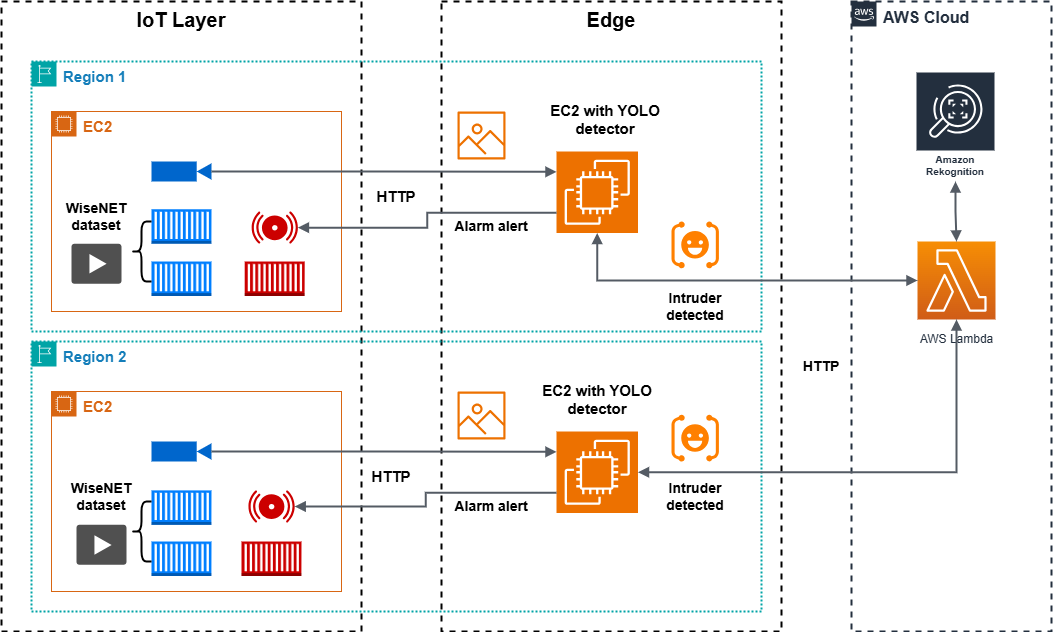
\includegraphics[width=1\linewidth]{res/report/DS_architecture_version2.png}
    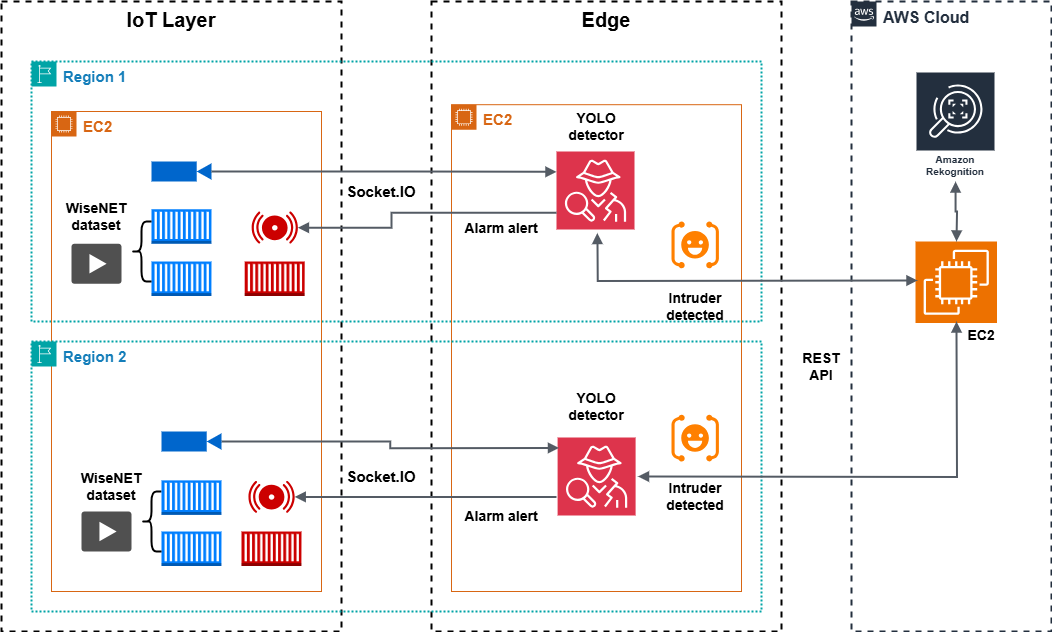
\includegraphics[width=1\linewidth]{DS_architecture_final.png}
    \caption{System architecture, depicting three separate layers in 2 regions}
    \label{fig:architecture}
\end{figure}

The edge layer also consists of an EC2 instance, simulating two distinct edge devices located in different areas. At the edge, the image stream is processed using the YOLO (You Only Look Once) algorithm. When a person-like object is detected, the relevant image snippet is forwarded to the cloud layer via a REST API and waits for a response. If a positive response is received, the edge triggers the alarm in the corresponding location. With sufficient resources in the cloud, the system can scale dynamically to meet demand.

The cloud layer integrates with Amazon Rekognition to perform facial recognition, comparing the detected face against a collection of known individuals. If an unknown person is identified, the cloud server triggers an alert, which is sent back to the edge device.

This architecture prioritizes performance and scalability. YOLO is used for fast, real-time object detection at the edge, minimizing latency. Amazon Rekognition handles facial recognition in the cloud, offloading computationally heavy tasks. WebSockets enable real-time, bidirectional communication for efficient image streaming with minimal delay. REST APIs ensure reliable data exchange, while EC2 instances simulate cameras and edge devices. 

\section{Implementation details}


\subsection{Layer implementation}
We decided that the IoT layer will consist of four camera containers and one alarm container for each edge device. This setup is an ideal simulation choice, as it minimizes the system’s computational requirements while maintaining the separation between individual devices. We use the WiseNET dataset (set\_3) for video simulation, which features two individuals appearing at different times—one simulating an intruder and the other an employee. The camera containers have access to the full set of videos, but each container selects one based on a container-specific environment variable, \textit{CAMERA}. The video sets are \textit{.avi} files that are read sequentially and looped when they reach the end.

We process these videos using OpenCV's \textit{read()} function to extract frame sequences. The system then transmits these frames at short intervals (1 second) to the edge device via the Socket.IO library. This significantly reduces the edge device's workload while maintaining low system latency. The alarm container maintains a connection to the edge server and remains in a waiting state until triggered by an event.\hfill \break

We implemented the edge layer as an EC2 instance running the YOLO (You Only Look Once) algorithm for object detection. The implementation is Python-based and utilizes OpenCV for frame processing. Each incoming image is analyzed for person-like objects. When such an object is detected, YOLO creates a snippet of the object and immediately forwards it to the cloud server via a REST API, ensuring a response. In the case of a positive detection, an alarm is triggered using Socket.IO for communication back to the IoT layer.\hfill \break

We let the cloud layer to focus on facial recognition and alert management through a REST API built using Python's Flask package to receive images from the edge layer. The system integrates directly with AWS Rekognition for facial recognition processing, with the Rekognition collection and known faces automatically provisioned at cloud server startup using boto3. Once processing is complete, the result is returned in the HTTP response. 

\subsection{Implementation Decisions}
In the software stack where several options were available and we decided to go for specific ones. This section provides rationale for the choices made. This includes the programming language, communication libraries and detection algorithms.
\\

\subsubsection{Communication}
The distributed system consists of several components that need to communicate in an efficient way - that's what makes it a distributed system. 
Namely two main interfaces need communictation:
\\
\begin{itemize}
    \item IOT - Edge communication
    \item Edge - Cloud communication
\end{itemize}

\hfill \break
For the \textbf{IOT - Edge} communication we decided to use socket.io. This Python library enables communication with websockets. As we need to send a constant stream of data, this communication model seems to be the best fit. The protocol includes a full-duplex communication channel build ontop of the network layer. Its a consistent communication model that requires minimal overhead for setting up the connection. 

This model handles many frames transfered very well and is very efficient. In comparision to HTTP that would require a new connection for every frame, this model is much more efficient. 
\\

%TODO: insert example of socket.io communication wit sockets.

For the \textbf{Edge - Cloud} communication we decided to use a REST API. This approach was implemented using Python's \textit{Flask} package to allow the distributed processing of the data. 

Our assumption for the choice of the communication model was that the data transfer between Edge and Cloud is not as frequent as between IOT and Edge. Ideally only a few requests per hour are sent to the cloud, as there are only few intruders in the office. When we would have tens of thousands of requests to the server per minute, we would argue there is something wrong in the office. 

Given our assumption, the overhead of setting up a new connection for every request is not as significant. Having a constant connection open to the cloud would be a waste of resources. 

The REST API is a stateless communication model that uses HTTP requests to transfer data. It is simple to implement and easy to understand. 

Whenever the preprocessing model (YOLO) detects a person in a frame, it sends the frame in a HTTP request to the cloud for further processing. 
The cloud immediately processes the image and sends the response back in the HTTP response. We efficiently use the request and respons for our computation. 
\hfill \break

\subsubsection{Dection Models}
In the system two detection models are used, namely: 
\begin{itemize}
\item YOLO: preprocessing images on Edge
\item AWS Rekognition: facial recognition on Cloud
\end{itemize}

\hfill \break

It was obvious to us to use Rekognition, as we already tested this AWS service in the course of the semester. It is a very powerful tool for facial recognition and very easy to use. 

YOLO was chosen as the detection model for the edge, as it is a very efficient object detection model. It is able to process images in real-time and is very accurate. There were multiple problems in setting up the model in Docker, especially with dependencies for the \textit{pytorch} library. We found a workaround using \textit{ultralytics} package, that wrappes \textit{torch} and special classes for YOLO into one package. Unfortunately the package is exceptionally big and exceeds the maximum image size of 1GB. We had no time to further optimize the size of the edge layer and decided to use the large image. 

YOLO and Rekognition can be easily encapsulated and used in the system. 
For example, we implemented a wrapper class for yolo usage, so we can use simply the \textit{yoloDetection.analyseImage(image)} function. 
Internally this function runs the yolo image detection, and returns True if a person was detected, otherwise False. 

\begin{center}
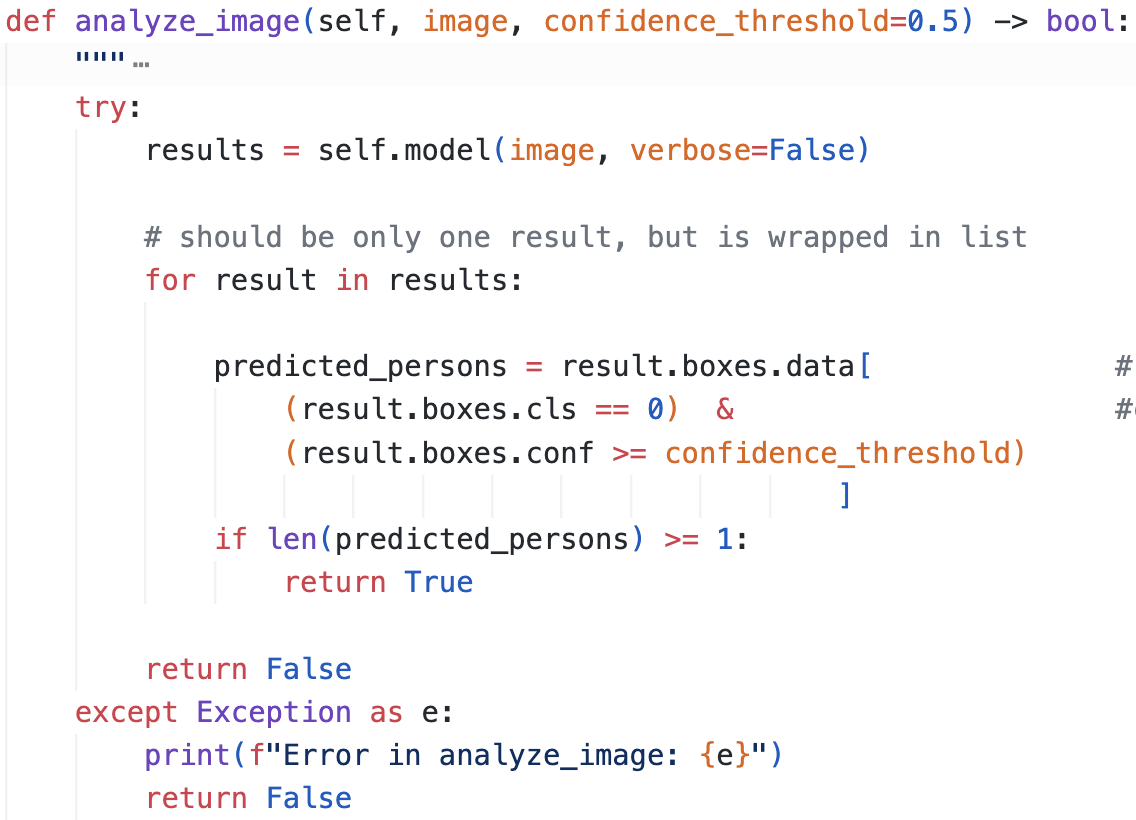
\includegraphics[width=1\linewidth]{analyze_image-function.png}
\end{center}

\section{Testing Setup}
In the first weeks of implementing the distributed system, we solely focused on simulating disjoint networks in Docker, utilizing the Docker-Networks feature. 

For every layer, we created a separate Dockerfile.[layer]. A simple \texttt{docker-compose.yaml} file was used to orchestrate the containers. In this orchestration, the camera containers were connected to the edge device, which in turn was connected to the cloud server. 
The IOT containers are connected to the same network as the edge, the edge in addition is connected to the cloud network. 
The following \textit{.yaml} shows the configuration for networking in docker containers.

\begin{verbatim}
networks:
  simulation_network:
    driver: bridge
  simulation_network_edge_cloud:
    driver: bridge

# then in the container specification: 
cloud: 
    build:
    context: .
    dockerfile: docker/Dockerfile.cloud
    image: cloud
    networks:
    # subscribe to the network
    - simulation_network_edge_cloud 
\end{verbatim}

This simple setup allowed us to test the communication between the layers and the correct processing of the data. 
Deployment was easy then, just a matter of spinning up the containers on the EC2 instances and adapting the IP addresses in the config file.

\section{Deployment Setup}
The entire distributed system runs on three AWS EC2 instances:
\begin{itemize}
    \item IOT - layer: camera instances
    \item EDGE - layer: edge instance with YOLO
    \item CLOUD - layer: cloud instance with AWS Rekognition
\end{itemize}

\hfill \break

The IoT layer components (4 camera containers and 1 alarm container) are consolidated on a single t2.micro instance, which is sufficient for simulating the video streams and alarm functionality.

The edge layer operates on a t2.medium instance. This increased computational capacity is necessary due to the resource demands of the YOLO algorithm for real-time person detection.

The cloud layer, hosting the AWS Rekognition integration and REST API, runs on a t2.micro instance, as the facial recognition processing is offloaded to AWS services.

This deployment configuration provides a cost-effective setup while ensuring adequate processing power where needed, particularly for the computationally intensive edge layer operations.

\begin{figure}[h!]
    \centering
    %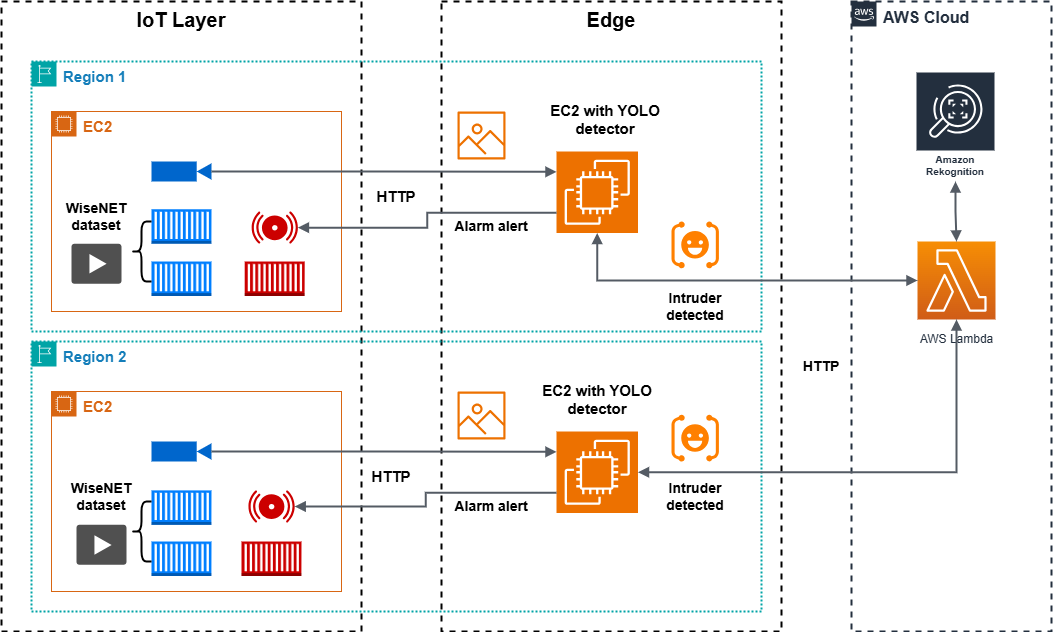
\includegraphics[width=1\linewidth]{res/report/DS_architecture_version2.png}
    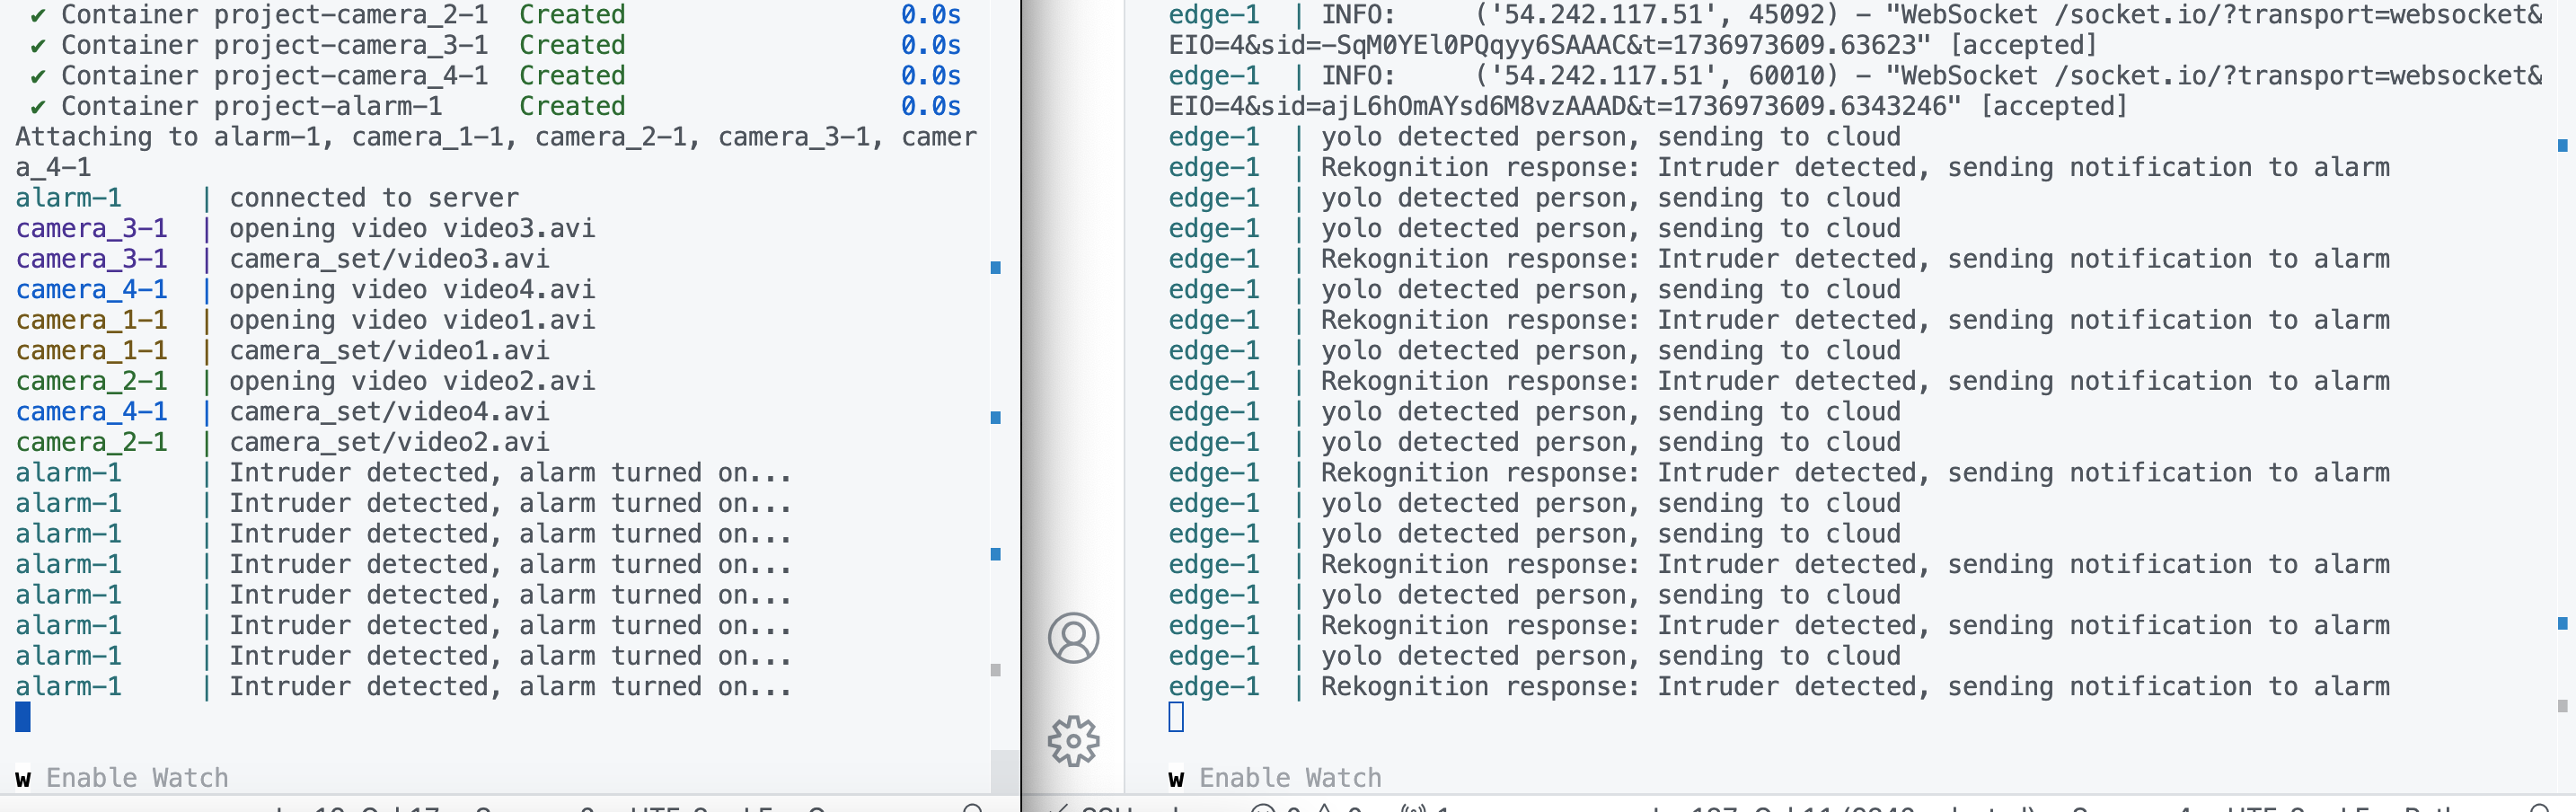
\includegraphics[width=1\linewidth]{deployment2.png}
    \caption{Sucessful detection of intruders.}
    \label{fig:deployment}
\end{figure}
\section{Evaluation}
Evaluation of the response time and scalability (number of devices and traffic) to prove the correctness of your implementation. The more detailed the better. 

\end{document}
